\documentclass{beamer}
\usepackage{graphicx}
\usepackage{animate}
\usepackage[mode=buildnew]{standalone}

\title{SURE Intern Progress Report: June 7-13}
\institute{Dynamic Adaptive Robotic Technologies Lab\\[\medskipamount]
\includegraphics[width= 0.6\textwidth, height=.25\textheight]{./images/dart_logo.png}}

\subtitle{Mark Jimenez}

\begin{document}

	\frame{
		\titlepage
	}
	\section{Progress}
	\frame{
		\frametitle{Dubins Motion Controller}
		\begin{columns}[T]
			\begin{column}{.5\textwidth}
			\begin{itemize}
				\item Hello
				\item World
			\end{itemize}
			\end{column}
			\begin{column}{.5\textwidth}

			\end{column}
		\end{columns}
	}
	\frame{
		\frametitle{Dubins Optimal Path Planner}
		\begin{columns}[T]
			\begin{column}{.5\textwidth}
			\end{column}
			\begin{column}{.5\textwidth}
				%\includestandalone[width=.8textwidth]{./tikz/dubins_curve}
				\includegraphics[width=\textwidth]{./tikz/dubins_curve.pdf}
			\end{column}
		\end{columns}
	}
	\frame{
		\frametitle{Optimal Planner vs. Controller}
		\begin{columns}[T]
			\begin{column}{.5\textwidth}
				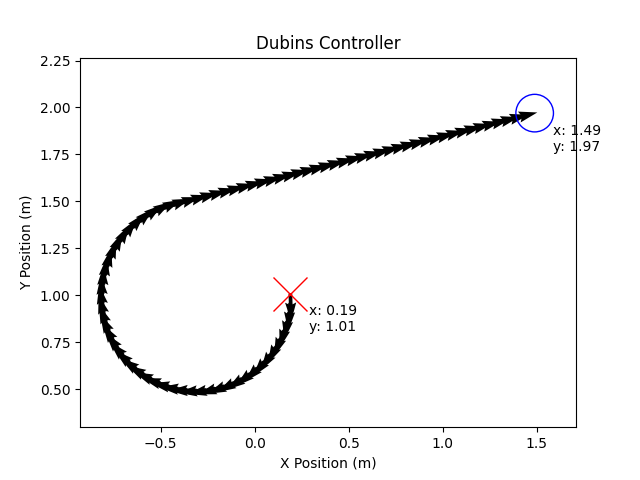
\includegraphics[width=\textwidth]{./images/dubins_steer_1}
				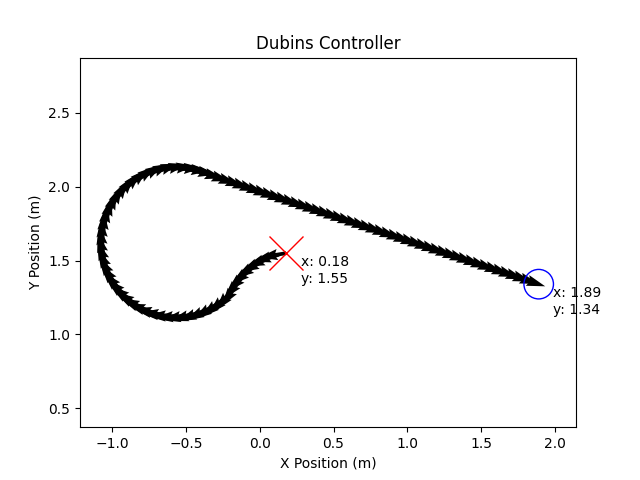
\includegraphics[width=\textwidth]{./images/dubins_steer_2}
			\end{column}
			\begin{column}{.5\textwidth}
				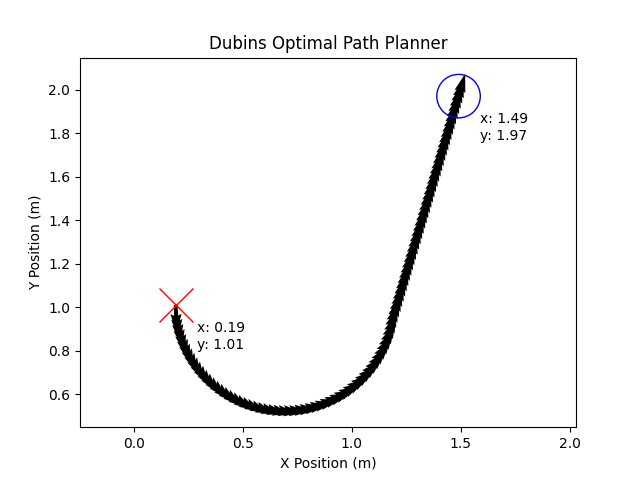
\includegraphics[width=\textwidth]{./images/dubins_optimal_1}
				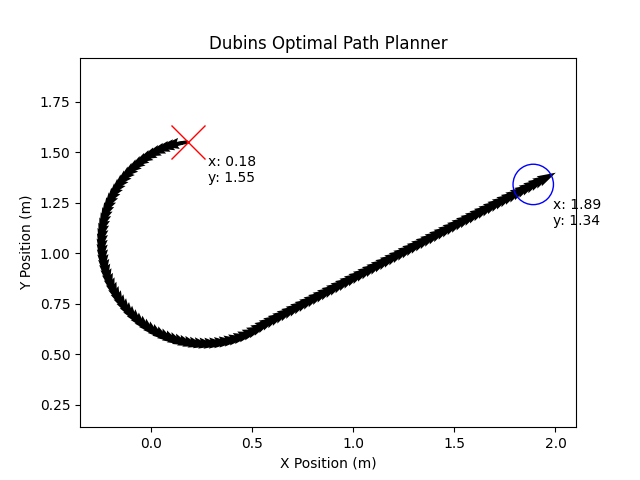
\includegraphics[width=\textwidth]{./images/dubins_optimal_2}

			\end{column}
		\end{columns}
	}
	\frame{
		\frametitle{Dubins Optimal Path Planner}
		\animategraphics[loop,controls,width=\linewidth]{10}{./images/optimal_planner_gif/optimal-}{0}{9}
	}
	\frame{
		\frametitle{RRT Algorithm}
	}
	\section{Next Steps}
	\frame{
		\frametitle{Data Generation}
	}
	\frame{
		\frametitle{Path-Target Classifier}
	}



\end{document}
